\documentclass[9pt,twocolumn,twoside]{../../styles/osajnl}
\usepackage{fancyvrb}
\journal{i524}

\title{Apache Crunch}

\author[1,*]{Scott McClary}

\affil[1]{School of Informatics and Computing, Bloomington, IN 47408, U.S.A.}

\affil[*]{Corresponding authors: scmcclar@indiana.edu}

\dates{paper-002, \today}

\ociscodes{Big-Data, Cloud, Hadoop, MapReduce}
\doi{\url{https://github.com/cloudmesh/sp17-i524/blob/master/paper2/S17-IO-3011/report.pdf}}

\begin{abstract}
Apache Crunch is a Java API that simplifies the process of developing
MapReduce pipelines. This library is built on top of Apache Hadoop and
Apache Spark and is therefore used in industry to develop efficient,
scalable and maintainable codebases for Big Data solutions. The main
benefit of Apache Crunch is that the explicit need to manage MapReduce
jobs has been abstracted away. Thus, Apache Crunch alleviates much of
the steep learning curve inherently within developing scalable
applications that utilize a MapReduce type approach.
\newline
\end{abstract}

\setboolean{displaycopyright}{true}

\begin{document}

\maketitle
\TODO{This review document is provided for you to achieve your
  best. We have listed a number of obvious opportunities for
  improvement. When improving it, please keep this copy untouched and
  instead focus on improving report.tex. The review does not include
  all possible improvement suggestions and if you sea comment you may
  want to check if this comment applies elsewhere in the document.}
\TODO{Please apply 80 character width for whatever editor you are using upon
your paper.}
\section{Introduction} \label{introduction}
Apache Crunch is an open source Java API that is ``built for pipelining MapReduce \CE programs which are simple and efficient'' \cite{www-hadoop-ecosystem}. More specifically, Crunch allows developers to write, test and run MapReduce pipelines with minimal upfront investment \cite{www-hadoop-ecosystem}.
\TODO{Even though two sentences come from the same reference, you don't
have to cite twice. The reference here
http://crunch.apache.org/source-repository.html
 is invalid. Shouldn't it be either
http://crunch.apache.org/index.html
or
http://crunch.apache.org/
?
}
As explained in Section \ref{about},
\TODO{This is not the correct way to do it. You can't say "As explained in" a
later section. Instead, you could say "This will be explained in a more detailed
way in the following section".}
this Java API was developed by Josh Wills at Cloudera \CE and is based on Google's FlumeJava library \cite{FlumeJava-paper-2012, www-crunch-about}.

Apache Crunch ``aims to make writing, testing, and running MapReduce pipelines easy, efficient, and even fun'' \cite{www-wills-crunch}. This open source Java API provides a ``small set of simple primitive operations and lightweight user-defined functions that can be combined to create complex, multi-stage pipelines'' \cite{www-wills-crunch}. Apache Crunch abstracts away much of the complexity from the user by compiling ``the pipeline into a sequence of MapReduce jobs and manages their execution'' \cite{www-wills-crunch}.
\subsection{Advantages}
As Hadoop continues to grow in popularity, the variation of data (i.e. satellite images, time series data, audio files, and seismograms) that is stored in HDFS \CE grows as well \cite{www-wills-crunch}. Many of these data ``formats are not a natural fit for the data schemas imposed by Pig \CE and Hive \CE;'' therefore, ``large, custom libraries of user-defined functions in Pig or Hive'' or ``MapReduces in Java'' have to be written, which significantly ``drain on developer productivity'' \cite{www-wills-crunch}. The Crunch API provides an alternative solution, which does not inhibit developer productivity. Apache crunch integrates seamlessly into Java and therefore, allow developers full access to Java to write functions. Thus, Apache Crunch is ``especially useful when processing data that does not fit naturally into relational model, such as time series, serialized object formats like protocol buffers or Avro records \CE , and HBase \CE rows and columns'' \cite{www-crunch-api}.

\begin{figure}[htbp]
\centering
\fbox{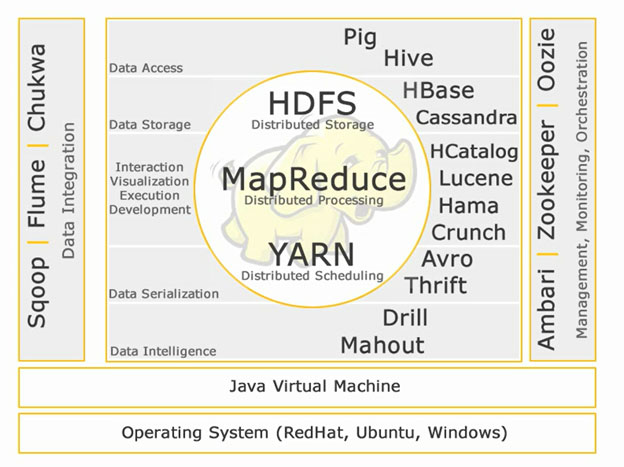
\includegraphics[width=\linewidth]{images/hadoop-ecosystem-and-components_3}}
\caption{The image above depicts the Apache Hadoop Ecosystem, including where Apache Crunch lies within the software stack \cite{www-hadoop-ecosystem}.}
\label{fig:hadoop-ecosystem-and-components_3}
\end{figure}

\subsection{About \& History} \label{about}
\TODO{The title here is not right. No one uses something like About \& History.
It can be just history.
Also, I am not sure why you put history after advantages. Shouldn't history
follow right after section introduction then following advantages?}
The major contributor to the ``initial source code of the Apache Crunch project [was] ... Josh Wills at Cloudera in 2011'' \cite{www-crunch-about}.
\TODO{What's the "[was] ..." about?}
Up until May 2012 (i.e. version 0.2.4), the Apache Crunch project was open sourced at GitHub \CE \cite{www-crunch-about}.
\TODO{
GitHub here needs citation.
} After May 2012, ``Cloudera donated the source code to Apache and the project entered the Apache Incubator, ... [a]fter 9 months at the Incubator, ...
\TODO{I am not sure what's ... [a]fter 9 months at the Incubator, ... here}
the Apache Board of Directors established the Apache Crunch project in February 2013 as a new top level project'' \cite{www-crunch-about}.
Since February 2013, the Apache Crunch project continues to be used, maintained and improved in an open source fashion, as explained in Section \ref{source}.
\TODO{Not appropriate}


\subsection{API} \label{api}
Apache Crunch is a Java API that is used ``for tasks like joining and
data aggregation that are tedious to implement on plain MapReduce''
\cite{www-crunch-api}. Section \ref{educational}
\TODO{Once again, not right}
explains that the
Apache Software Foundation provides thorough documentation of the API
and provides examples of how to explicitly leverage this API from a
Java application.

\subsubsection{Shell Access} \label{shell}
For users of the Scala programming language, there is the ``Scrunch
API, which is built on top of the Java APIs and includes a REPL
(read-eval-print loop) for creating MapReduce pipelines''
\cite{www-crunch-api}.

\section{Licensing} \label{licensing}
The Apache Software Foundation, which includes Apache Crunch, is
licensed under the Apache License, Version 2.0 \cite{www-apache-lic}.

\subsection{Source Code}\label{source}
Apache Crunch leverages Git \CE for version control, which allows the user
and developer communities to contribute freely to this open source
project \cite{www-crunch-git}.

\section{Architecture \& Ecosystem} \label{ecosystem}
Figure \ref{fig:hadoop-ecosystem-and-components_3} and Figure
\ref{fig:architecture} provide a complete graphical representation of
the MapReduce ecosystem and explicitly indicates Apache Crunch's place
within the software stack. In the simplest of terms, Apache Crunch
runs on top of Hadoop MapReduce and Apache Spark
\cite{www-crunch-api}.
\TODO{You can't just put two content rich figures within your paper without
any explanation. You either explain your figure or you don't put anything here.}
\begin{figure}[htbp]
\centering
\fbox{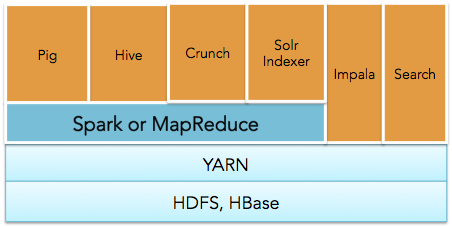
\includegraphics[width=\linewidth]{images/hadoop-architecture}}
\caption{The image above depicts the Apache Hadoop software stack, including Apache Crunch \cite{www-crunch-architecture}.}
\label{fig:architecture}
\end{figure}


\section{Use Cases} \label{use}
Apache Crunch has its applicability in the Big Data industry, as shown
in Section \ref{big}. The widespread usage of Apache Hadoop and Apache
Spark help to promote Apache Crunch in industry and academia alike.

\subsection{Use Cases for Big Data} \label{big}
As explained in Section \ref{ecosystem}, Apache Crunch is built on top
of Hadoop MapReduce and Apache Spark, which both go hand in hand in
solving many complicated and challenging Big Data problems.

\subsection{Cerner} \label{cerner}
Cerner, ``an American supplier of health information technology (HIT)
solutions, services, devices and hardware'' \cite{www-cerner}, employs
Apache Crunch to solve many of their Big Data problems
\cite{www-crunch-cerner}. Cerner chose to use Apache Crunch since it
interestingly solves what they refer to as ``a people problem''
\cite{www-crunch-cerner}. As a company, they have noticed that Apache
Crunch diminishes a potential steep learning curve for new employees
and/or teams to use Big Data technologies. Specifically, Apache Crunch
stands above the other ``options available for processing pipelines
including Hive, Pig, and Cascading'' since Apache Crunch allows Cerner
employees to ``easily ... translate how [they] ...
\TODO{Once again, not right here.}
described a problem
into concepts [that they] ... can code'' \cite{www-crunch-cerner}. The
diminished learning curve as a result of using Apache Crunch allows
Cerner to focus their time, effort and money on performance tuning
and/or algorithm adjustments rather than spending a significant amount
time simply translating the problem into runnable code
\cite{www-crunch-cerner}.

\subsection{Spotify} \label{spotify}
Spotify, the popular ``music, podcast, and video streaming service''
\cite{www-spotify}, leverages Apache Crunch to process the many
terabytes of data generated every day by their large user community
\cite{www-crunch-spotify}. Spotify has been using Hadoop since 2009
and have spent significant effort since then to develop tools that
make it ``easy for [their] developers and analysts to write data
processing jobs using the MapReduce approach in Python''
\cite{www-crunch-spotify}. However, in 2013 Spotify came to the
realization that this approach wasn't performing well enough so they
decided to start using Java and Apache Crunch to solve their Big Data
problems \cite{www-crunch-spotify}. This transition to Apache Crunch
resulted in higher performance, higher-level abstractions (e.g.
filters, joins and aggregations), pluggable execution engines
(e.g. MapReduce and Apache Spark) and added simple powerful testing
(e.g. fast in-memory unit tests) \cite{www-crunch-spotify}. Apache
Crunch has given Spotify a ``huge boost for both [their] ... developer
\TODO{Not right.}
productivity and execution performance on Hadoop''
\cite{www-crunch-spotify}.

\section{Educational Material} \label{educational}
Apache Crunch makes the process of developing applications that
leverage MapReduce and Apache Spark easier; therefore, the learning
curve is much less significant in relation to developing applications
that directly interact with MapReduce and Apache Spark. The Apache
Software Foundation provides a lot of useful documentation. For
instance, there is API documentation \cite{www-apache-docs} as well as
getting started information \cite{www-crunch-started}, a user guide
\cite{www-crunch-user-guide} and even source code installation
information \cite{www-crunch-git}. If this is not enough, complete and
extensive third-party code examples explain how to develop ``hello
world'' applications that use Apache Crunch
\cite{www-crunch-tutorial}.

\section{Conclusion} \label{conclusion}
In general, Apache Crunch simplifies the process of writing and
maintaining large-scale parallel codes by abstracting away the need to
manage MapReduce jobs. This abstraction diminishes the inherent
learning curve in solving Big Data problems and therefore allows
developers to focus their time and effort in developing the general
concept of their solution rather than in the detailed process of
writing their code. The aforementioned benefits of Apache Crunch are
proven by its widespread use in industry (e.g. Spotify and Cerner) and
in academia, shown in Section \ref{use}.

\TODO{The content here is a little bit too short to me considering two large
figures within. I would suggest to talk a little more about architecture since
you have included the figure.}
\section*{Acknowledgements}
The authors would like to thank the School of Informatics and
Computing for providing the Big Data Software and Projects (INFO-I524)
course \cite{www-i524}. This paper would not have been possible
without the technical support \& edification from Gregor von Laszewski
and his distinguished colleagues.


\section*{Author Biographies}
\begingroup
\setlength\intextsep{0pt}
\begin{minipage}[t][3.2cm][t]{1.0\columnwidth}
  \begin{wrapfigure}{L}{0.25\columnwidth}
    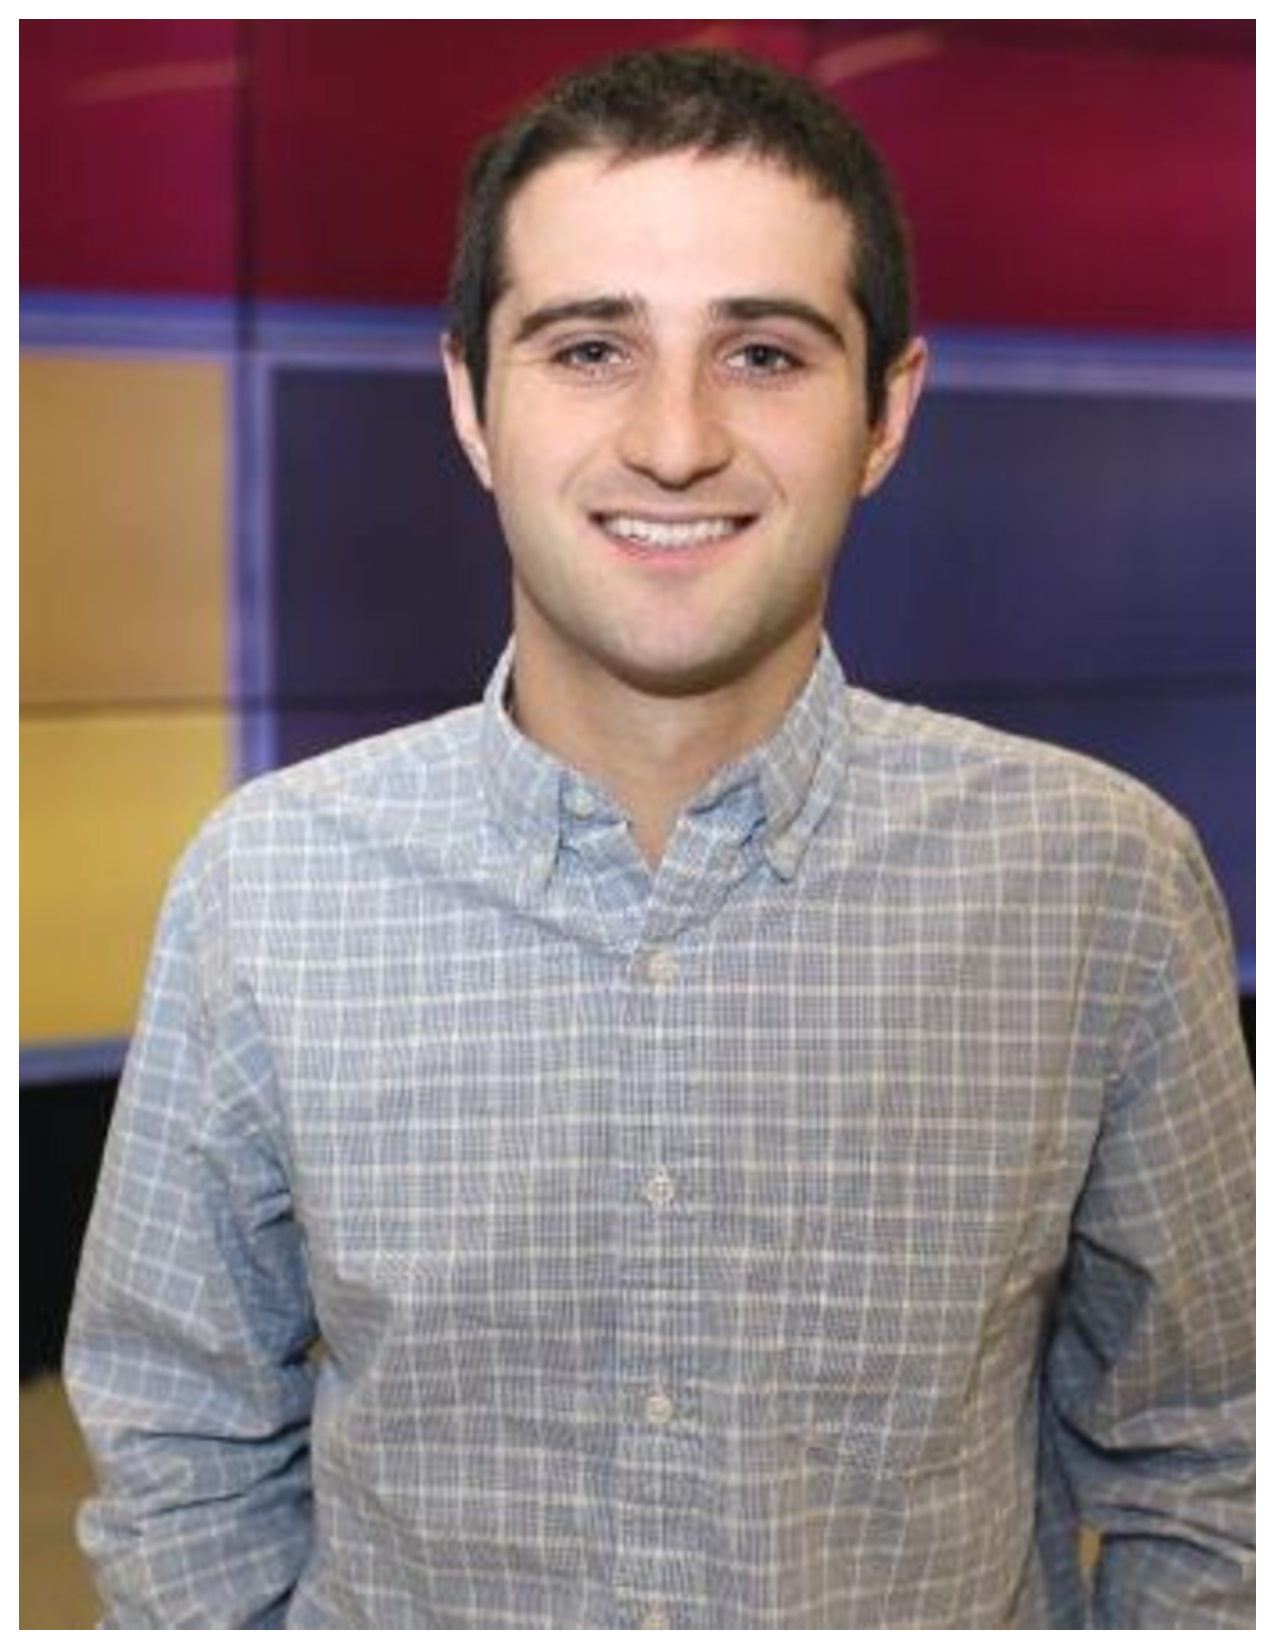
\includegraphics[width=0.25\columnwidth]{images/scott_mcclary}
  \end{wrapfigure}
  \noindent
  {\bfseries Scott McClary} received his BSc (Computer Science) and
  Minor (Mathematics) in May 2016 from Indiana University and will
  receive his MSc (Computer Science) in May 2017 from Indiana
  University. His research interests are within scientific application
  performance analysis on large-scale HPC systems. He will begin
  working as a Software Engineer with General Electric Digital in San
  Ramon, CA in July 2017.
\end{minipage}
\endgroup

\section*{} %used to create a little more spacing..
\section*{Work Breakdown}
The work on this project was distributed as follows between the
authors:
\begin{description}
\item[Scott McClary.] He completed all of the work for this paper
  including researching and testing Apache Airavata as well as
  composing this technology paper.
\end{description}

% Bibliography
\bibliography{references}
\end{document}
